\documentclass[a4paper,11pt]{article}
%%%%%%%%%%%%%%%%%%%%%%%%%%%%%%%%%%%%%%%%%%%%%%%%%%%%%%%%%%%%%%%%%%%%%%%%%%%%%%%%
\usepackage{ccs_iogs}
%%%%%%%%%%%%%%%%%%%%%%%%%%%%%%%%%%%%%%%%%%%%%%%%%%%%%%%%%%%%%%%%%%%%%%%%%%%%%%%%
\begin{document}

\newpage
\begin{minipage}[c]{.25\linewidth}
	
\includegraphics[width=4cm]{images/LEnsE_IOGS.jpg}
\end{minipage} \hfill
\begin{minipage}[c]{.4\linewidth}

\begin{center}
\vspace{0.3cm}
{\Large OPTO-ELECTRONIQUE}

\medskip

\textbf{\Large TP Séance 6 / AM}

\end{center}
\end{minipage}\hfill

\begin{center}
\vspace{0.3cm}

\noindent \rule{\linewidth}{1pt}

Durée : 3h / Modulation et Démodulation / Détection synchrone

\vspace{-0.2cm}
\noindent \rule{\linewidth}{1pt}
\end{center}


%%%%%%%%%%%%%%%%%%%%%%%%%%%%%%%%%%
\section*{Objectifs de l'expérience}

On se propose dans ce TP de réaliser une \textbf{démodulation d'un signal modulé en amplitude}, à partir d'une détection synchrone pré-câblée (Partie A) et de réaliser la \textbf{transmission} de ce signal par fibre optique (Partie B).

On réalisera un \textbf{étage actif de filtrage} (Partie C) permettant de récupérer le signal modulant.

\subsection*{Description de la maquette}

On se propose dans cette séance d'étudier la maquette suivante permettant de faire de la modulation et de la démodulation, ainsi que de la transmission par fibre optique.

On donne le schéma fonctionnel suivant :

	\begin{center}
		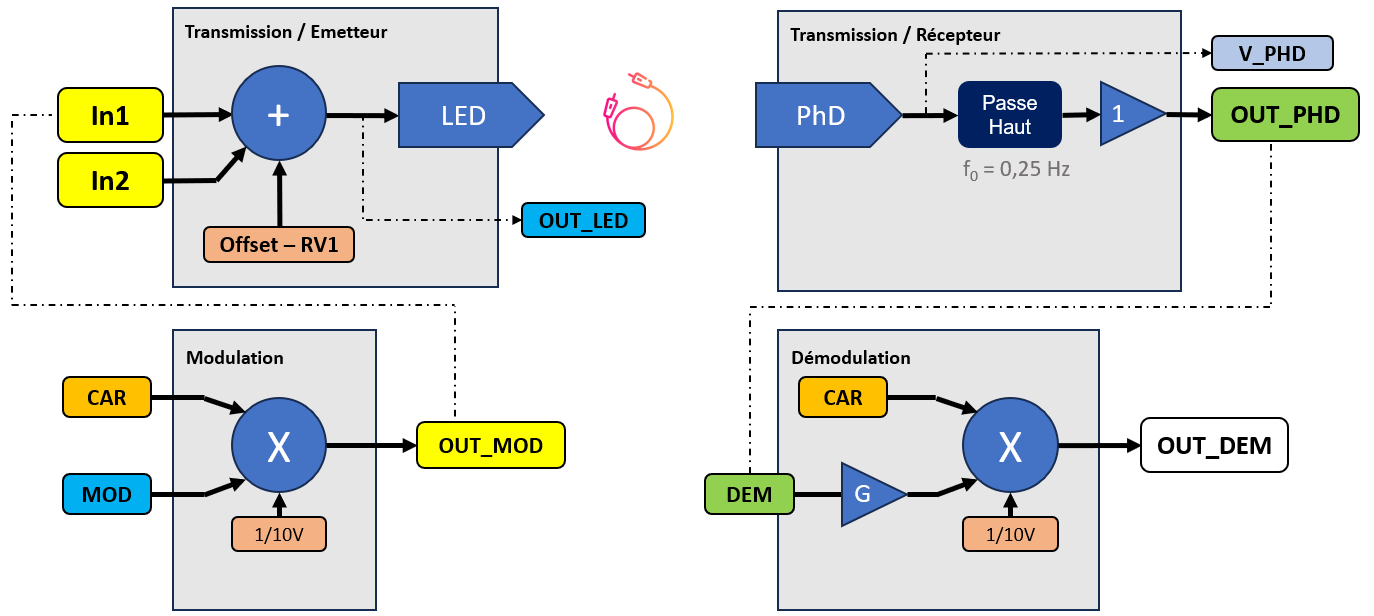
\includegraphics[width=0.9\textwidth]{images/AM_modulation.png}
	\end{center}


L'entrée \textbf{MOD} correspond à la modulante, soit $V_m(t)$ (fréquence lente), et l'entrée \textbf{CAR} correspond à la porteuse, soit $V_p(t)$ (fréquence rapide).

L'entrée \textbf{DEM} correspond au signal modulé.

\bigskip

\textit{On donne également le schéma du circuit électronique complet en annexe à ce document.}

	
\newpage
\section*{Partie A - Etude de la modulation/démodulation \textsc{\normalsize(Durée conseillée : 90 min)}}


%%%%%%%%%%%%%%%%%%%%%%%%%%%%%%%%%%
\subsection*{Etude théorique de la modulation en amplitude}

On s'intéresse à l'étage \textbf{Modulation} de la maquette.

On appellera la \textbf{modulante} \fbox{MOD} le signal $V_m(t) = A_m \cdot sin(2 \cdot \pi \cdot f_m \cdot t + \phi_m)$ (fréquence lente) sur  \textsc{\textbf{IN1}} et la \textbf{porteuse} \fbox{CAR} le signal $V_p(t) = A_p \cdot sin(2 \cdot \pi \cdot f_p \cdot t + \phi_p)$ (fréquence rapide).

On supposera que $f_p >> f_m$.

\bigskip

\Real Quel signal obtient-on sur la sortie \fbox{OUT\_MOD} ? Expliquer en quoi cela correspond à une \textbf{modulation d'amplitude}. 

\Real Quel spectre attend-on pour le signal de sortie OUT\_MOD ?


%%%%%%%%%%%%%%%%%%%%%%%%%%%%%
\subsection*{Mise en oeuvre de l'étage de modulation}

La maquette nécessite une alimentation symétrique de +$V_{CC}$ / -$V_{CC}$. On choisira $V_{CC} = 10~V$).

\medskip

\Real Proposer un protocole pour valider le fonctionnement de l'étage de modulation. On s'intéressera en particulier aux composantes fréquentielles incluses dans ce signal de sortie (par rapport aux fréquences des signaux d'entrée - FFT).

\Real Mettre en oeuvre ce protocole et montrer le fonctionnement de l'ensemble.

\Real Analyser les caractéristiques des signaux de sortie.


%%%%%%%%%%%%%%%%%%%%%%%%%%%%%%%%%%
\subsection*{Etude théorique de la démodulation}

On s'intéresse à présent à l'étage de \textbf{démodulation}.

Le signal modulé précédent est appliqué sur l'entrée \fbox{DEM} de l'étage de démodulation. Le signal \fbox{CAR} est le même signal porteur que précédemment.

\Real Quel signal obtient-on sur la sortie \fbox{OUT\_DEM} ? Quel spectre attend-on pour le signal de sortie OUT\_DEM ?

\Real Expliquer comment récupérer alors le signal modulant initial.

\textit{Le principe utilisé ici est appelé \textbf{détection synchrone}.}


\subsection*{Mise en oeuvre de l'étage de démodulation}

\Real Proposer un protocole pour valider le fonctionnement de l'étage de modulation. On s'intéressera en particulier aux composantes fréquentielles incluses dans ce signal de sortie (par rapport aux fréquences des signaux d'entrée - FFT).

\Real Mettre en oeuvre ce protocole et montrer le fonctionnement de l'ensemble.

\Real Analyser les caractéristiques des signaux de sortie, en particulier les composantes fréquentielles des différents signaux mis en jeu.


\newpage
%%%%%%%%%%%%%%%%%%%%%%%%%%%%%%%%%%
%%%%%%%%%%%%%%%%%%%%%%%%%%%%%%%%%%
%%%%%%%%%%%%%%%%%%%%%%%%%%%%%%%%%%
\section{Partie B - Transmission par fibre \textsc{\normalsize(Durée conseillée : 60 min)}}

\Real Rappeler la caractéristique statique d'une LED et les zones de fonctionnement de ce composant. 

On se propose d'étudier la structure autour de l'\textbf{amplificateur U4A} (schéma donné en annexe).

\Real Donner la relation existante entre la sortie de l'amplificateur U4A - \fbox{OUT\_LED} - et les entrée \fbox{IN1}, \fbox{IN2} et \fbox{Offset}. \textit{On pourra supposer que $R_7$ est infinie pour le calcul.}

Ce signal est ensuite appliqué sur la LED d'émission protégée par la résistance $R_1$.

\Real A quoi sert la tension \fbox{Offset} modifiable par l'intermédiaire du potentiomètre RV1 ?

%%%%%%%%%%%%%%%%%%%%%%%%%%%%%
\subsection*{Mise en oeuvre de l'étage d'émission}

\Real Appliquer :
\begin{itemize}
	\item sur l'entrée \fbox{IN1} : un signal sinusoïdal de fréquence 1kHz, d'amplitude 1V et de valeur moyenne nulle
	\item sur l'entrée \fbox{IN2} : un signal triangulaire de fréquence 10kHz, d'amplitude 1V et de valeur moyenne nulle
\end{itemize}

\Real Visualiser le signal \fbox{OUT\_LED} pour différente position du potentiomètre RV1. Correspond-il au signal attendu ?


%%%%%%%%%%%%%%%%%%%%%%%%%%%%%
\subsection*{Etude du signal transmis / Récepteur}

\Real Rappeler la caractéristique statique d'une photodiode et les zones de fonctionnement de ce composant. Expliquer le principe de photodétection utilisé sur cette maquette et le rôle des éléments ajoutés après la photodiode dans le schéma proposé en annexe.

\Real Visualiser le signal \fbox{V\_PHD}. Ajuster la tension de sortie du potentiomètre RV1 pour obtenir un signal exploitable.

\Real Visualiser le signal \fbox{OUT\_PHD}. Expliquer les caractéristiques de ce signal.


\newpage
%%%%%%%%%%%%%%%%%%%%%%%%%%%%%%%%%%
%%%%%%%%%%%%%%%%%%%%%%%%%%%%%%%%%%
%%%%%%%%%%%%%%%%%%%%%%%%%%%%%%%%%%
\section{Partie C - Filtrage analogique \textsc{\normalsize(Durée conseillée : 90 min)}}

On se propose d'étudier un filtre actif basé sur la structure suivante :

\begin{center}
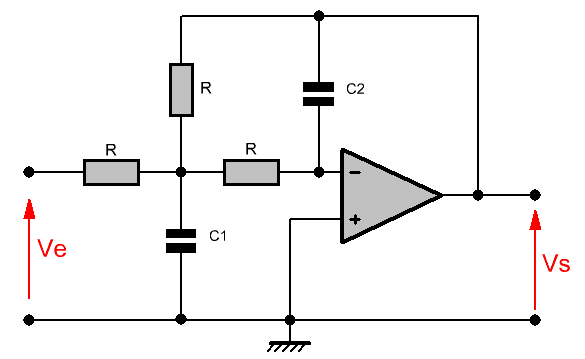
\includegraphics[scale=0.75]{images/rauch.png}
\end{center}

La pulsation caractéristique de ce filtre vaut $\omega_c = \frac{1}{R \cdot \sqrt{C_1 C_2}}$ et le facteur de qualité vaut $Q = \frac{1}{3} \cdot \sqrt{\frac{C_1}{C_2}}$.


\textbf{\textsc{On utilisera l'alimentation symétrique précédente ($V_{CC} = 10V$).}}	



%%%%%%%%%%%%%%%%%%%%%%%%%%%%%%%%%%
\subsection*{Etude théorique}

Ce montage utilise un amplificateur linéaire intégré (ALI) de type \texttt{TL071}/\texttt{TL081}.

\Real Faire une étude du fonctionnement du circuit en basse et en haute fréquence. En déduire le comportement attendu de ce filtre et donner les valeurs numérique le caractérisant pour les valeurs de composants
suivantes : $R = 2.2\operatorname{k\Omega}$, $C_1 = 22\operatorname{nF}$ et $C_2 = 2.2\operatorname{nF}$.

%%%%%%%%%%%%%%%%%%%%%%%%%%%%%%%%%%
\subsection*{Etude en fréquence de cette structure}

\Real Réaliser le montage précédent. 

\Real Proposer un protocole d'étude en fréquence de ce montage.

\Real Caractériser ce système pour des fréquences allant de 10Hz à 100kHz.

\Real Analyser les résultats pour valider le comportement de ce filtre.


\subsection*{Montage complet}

\Real Justifier le rôle du filtre vis-à-vis du système de détection synchrone pour récupérer le signal modulant. Comment mettre en cascade les différents éléments pour retrouver le signal modulant initial ?

\Real Valider le principe de la démodulation en associant tous les montages.



%%%%%%%%%%%%%%%%%%%%%%%%%%%%%%%%%%

\noindent \rule{\linewidth}{1pt}



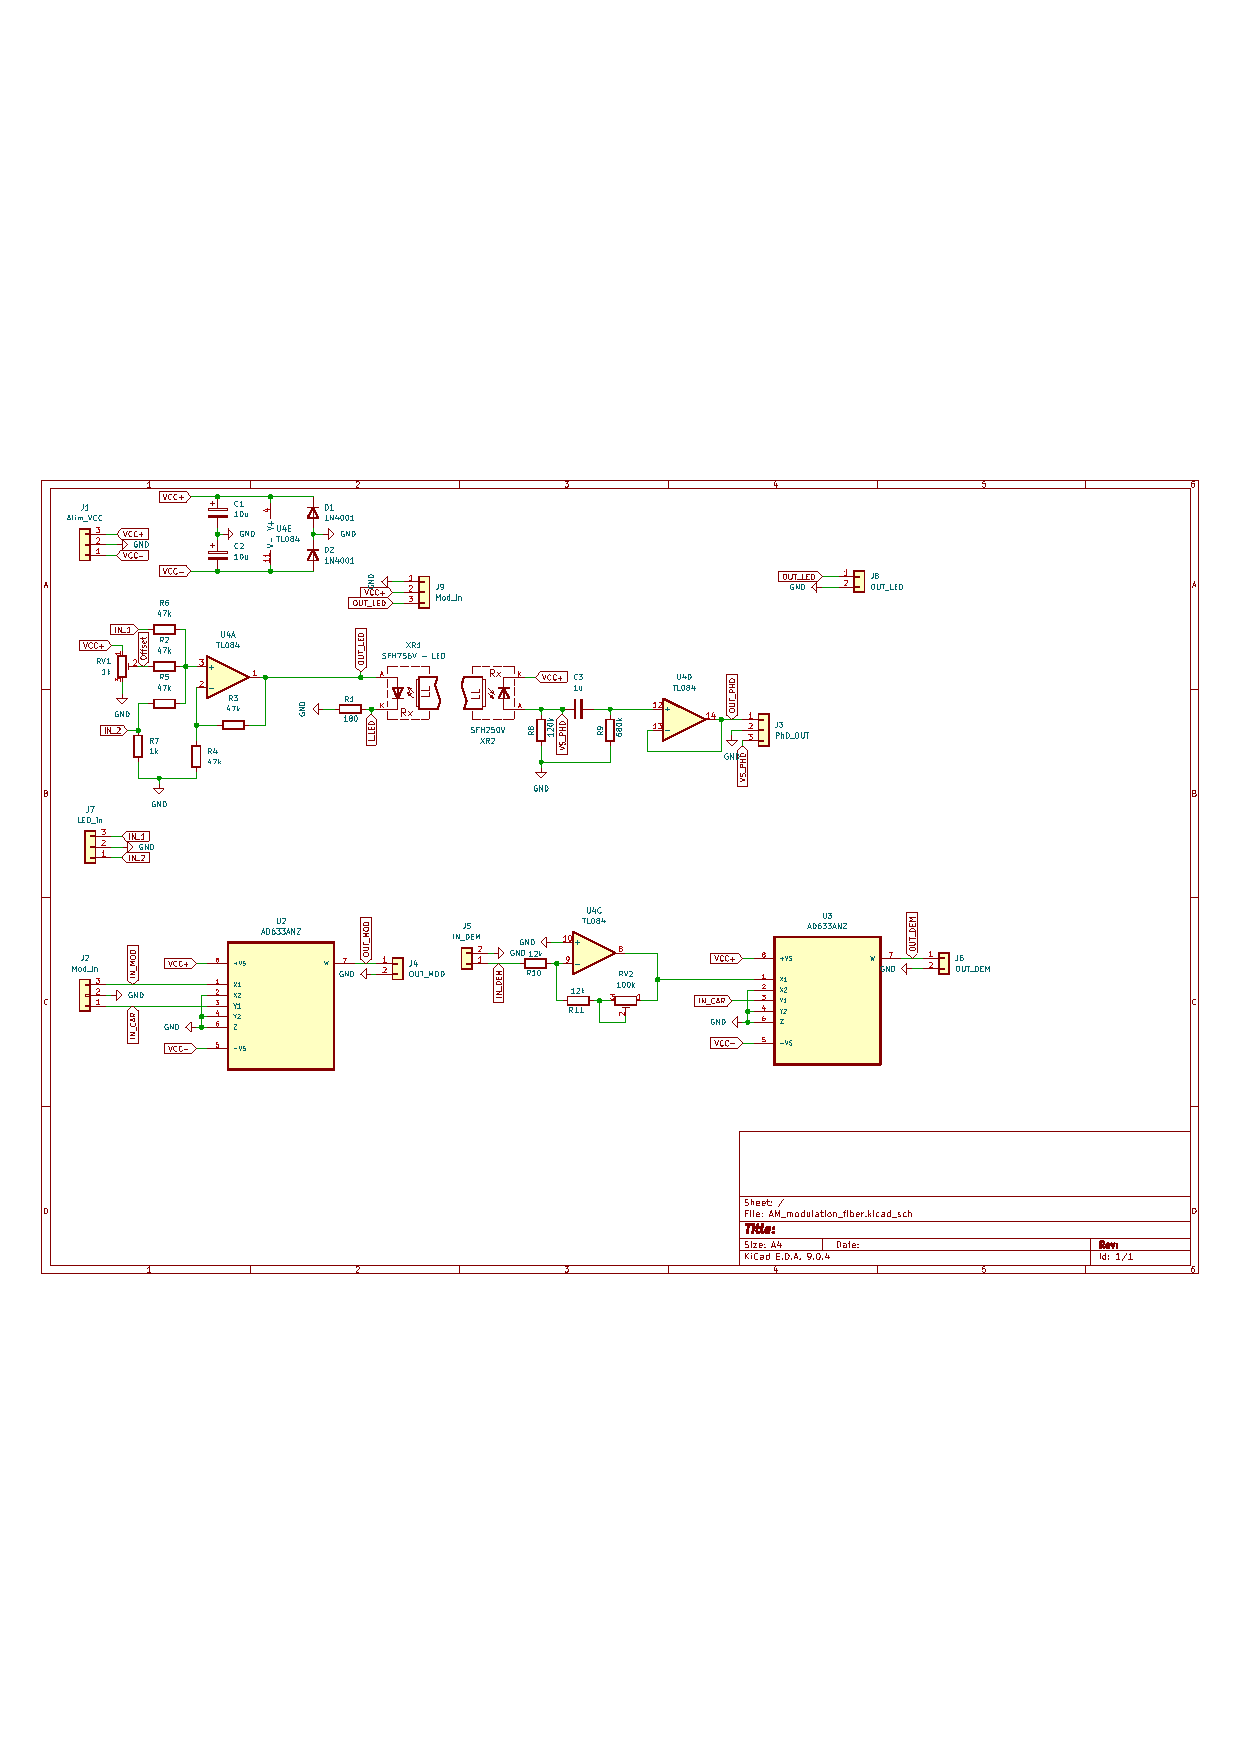
\includepdf[pages=-,landscape=true]{docs/AM_modulation_schema.pdf}


\end{document}
